\chapter{Oversubscription Planning}\label{ch:osp}
%\chapterquote{Having conflicting goals, dedicating resources to unconnected targets, and accommodating incompatible interests [...] make for bad strategy.}{...}
\chapterquote{A goal is not always meant to be reached, it often serves simply as something to aim at.}{Bruce Lee}

\renewcommand{\kiviatGoal}{2}
\begin{figure}[t]
    \begin{center}
        \begin{tikzpicture}
    \tkzKiviatDiagram[
    radial style/.style ={-{Latex[length=3mm, width=2mm]}},
    scale=0.85,
    label space=1.5,
    radial = 1,
    gap = 1.5,
    step = 1,
    lattice = 2]{
    \hspace{2.5cm}\mbox{\parbox{4cm}{{\begin{center}\textbf{Goal}\\\textbf{Description} \end{center}}}},
    {\textbf{Number of Plans}},
    \hspace{-1.5cm}\mbox{\parbox{3cm}{{\begin{center}\textbf{State}\\\textbf{Description}\end{center}}}},
    \textbf{Cost Function}}

    \ifbool{kiviatRed}{
        \tkzKiviatLine[very thick,color=red!50,
            fill=red!30,
            opacity=.35,
            mark=ball,
            mark size=2.5pt,
            ball color=red](\kiviatGoal{},\kiviatTopk{},\kiviatPredicates{},\kiviatCost{})
    }

    \ifbool{kiviatBlue}{
        \tkzKiviatLine[very thick,color=blue!50,
            fill=blue!30,
            opacity=.35,
            mark=ball,
            mark size=2.5pt,
            ball color=blue](1,1,1,1)
    }

    \ifbool{kiviatFull}{
    \tkzKiviatLine[very thick,color=darkgreen!50,
        fill=green!30,
        opacity=.35,
        mark=ball,
        mark size=2.5pt,
        ball color=darkgreen](1,2,2,2)
    \tkzKiviatLine[very thick,color=blue!50,
        fill=blue!30,
        opacity=.35,
        mark=ball,
        mark size=2.5pt,
        ball color=blue](1,1,1,1)
    \tkzKiviatLine[very thick,color=red!50,
        %fill=red!30,
        %opacity=.35,
        mark=ball,
        mark size=2.5pt,
        ball color=red](\kiviatGoal{},\kiviatTopk{},\kiviatPredicates{},\kiviatCost{})
    \LegendBox[shift={(-0cm,-2.25cm)}]{current bounding box.south west}%
    {
    red!100/{Forward symbolic search (contribution of this thesis)},
    asparagus!100/{Bidirectional symbolic search (contribution of this thesis)},
    blue!100/{Bidirectional symbolic search (previous state of the art)}}
    }
    {}

    % goal specification
    \draw[] node[align=center,fill=none] at (1.5,-0.5) {\small Hard};
    \draw[] node[align=center,fill=none] at (3.25,-0.75) {\small Oversub-\\ \small scription};
    %\draw[] node[] at (1.75,-0.6) {\rotatebox{-45}{hard}};
    %\draw[] node[align=center] at (3.85,-1.25) {\rotatebox{-45}{oversubscription}};

    % number of plans
    \draw[] node[align=center,fill=none] at (0.7,1.5) {\small Top-$1$};
    \draw[] node[align=center,fill=none] at (0.7,3.0) {\small Top-$k$};

    % derived predicates
    \draw[] node[align=center,fill=none] at (-1.25,0.75) {\small State\\ \small Variables};
    \draw[] node[align=center,fill=none] at (-3.25,0.75) {\small $+$ \small Derived\\ \small Variables};

    % cost function
    \draw[] node[align=center,fill=none] at (-1,-1.5) {\small Constant};
    \draw[] node[align=center,fill=none] at (-1.6,-3.0) {\small State-Dependent\phantom{0}};
\end{tikzpicture}
    \end{center}
    \caption[Overview of extension for classical planning (goal description).]{Overview of extensions for classical planning, where the red color denotes the planning formalism supported by the proposed symbolic search approach.}
    \label{fig:goal_description:kiviat}
\end{figure}
\renewcommand{\kiviatGoal}{1}

\section*{Core Publication of this Chapter}
\renewcommand{\citebf}[1]{\textbf{#1}}
\begin{itemize}
    \item \fullcite{speck-katz-aaai2021}
\end{itemize}
\renewcommand{\citebf}[1]{#1}

In conventional classical planning, goal states are defined by a goal condition, which is treated as a hard constraint that must be fully satisfied by any solution/plan.
In many real-world applications, however, the description of goals is oversubscribed, i.e., there are a large number of desirable, often competing goals of varying value, and a system (e.g., a Mars rover) may
not be able to achieve all of them with the available resources (e.g., battery power).
In such scenarios, it is natural to assign different utility values to states and to search for feasible and achievable states that maximize the overall utility value.
This planning formalism is called \emph{partial satisfaction planning}. Here, we distinguish between \emph{net-benefit planning} \autocite{vandenbriel-et-al-aaai2004}, where operator costs and state utility values, i.e., solution costs and solution utilities, are comparable, and \emph{oversubscription planning} \autocite{smith-icaps2004}, where those are not comparable. 

Symbolic search in the context of partial satisfaction planning has been studied to a limited extent.
For net-benefit planning, symbolic branch-and-bound search was introduced \autocite{edelkamp-kissmann-ijcai2009,kissmann-phd2012}, which considers so-called soft-goal planning tasks, i.e., planning tasks in which the utility function is a weighted sum over a subset of the state variables. 
Since \textcite{keyder-geffner-jair2009} provided a simple and concise compilation from net-benefit planning (soft-goal planning tasks) to classical planning, which is most commonly used in practice, we will focus on oversubscription planning, which is considered more challenging \autocite{domshlak-mirkis-jair2015}.
%
For oversubscription planning, there are a variety of explicit (heuristic) search approaches, mainly based on adapting existing heuristics from classical planning to oversubscription planning \autocite{mirkis-domshlak-icaps2013,domshlak-mirkis-jair2015,muller-karpas-icaps2018,katz-et-al-icaps2019,katz-et-al-icaps2019,garcia-olaya-et-al-aij2021}.
An important example of symbolic search in the context of oversubscription planning is the work of \textcite{eifler-et-al-ijcai2020}, in which plan explanations were investigated considering plan utilities.
The work of \textcite{speck-katz-aaai2021} is the first to explicitly define and study in detail symbolic search for solving oversubscription planning problems.
%To the best of our knowledge, \textcite{speck-katz-aaai2021} were the first to explicitly define and investigate symbolic search directly for solving oversubscription planning problems.

In this chapter, we define and motivate oversubscription planning that allows to extend the goal specification (\Cref{fig:goal_description:kiviat}), and discuss and summarize complexity and compilability results for this setting.
Then, an optimal and complete symbolic search approach for oversubscription planning introduced by \textcite{speck-katz-aaai2021} is presented.
The empirical analysis shows that the presented symbolic approach competes favorably with explicit heuristic state-space search.

\section{Formalism}

We consider oversubscription planning tasks \autocite{smith-icaps2004,katz-et-al-icaps2019}, where the solution cost and utility are \emph{not comparable}.

\begin{definition}[Oversubscription Planning]\label{def:planning_osp}
    An \emph{oversubscription planning (osp) task} is a tuple $\task = \langle \domain, \init, \goal, \limit \rangle$ with $\domain = \langle \vars, \operators, \constcostfun, \utility\rangle$ that extends an ordinary planning task and domain by a state utility function $\utility : \states \to \mathbb{N}_0$ that assigns utility to states.
\end{definition}

Similar to planning with sdac, where we focused mainly on cost functions that can be evaluated in polynomial time, here we focus mainly on utility functions that can be evaluated in polynomial time.
We assume that the utility function $\utility$ has the same form as an operator cost function (\Cref{def:cost-function}).

Since we consider utility in osp, it is natural to search for a plan that maximizes utility, i.e., leads to a state with high utility within the cost bound $\limit$. For this purpose, we define an osp plan as follows and introduce the concept of utility-optimal plans.

\begin{definition}[Osp Plan]\label{def:osp_plan}
    An \emph{(osp) plan} $\pi$ is defined as an ordinary classical plan (\Cref{def:plan}), i.e., an applicable sequence of operators that leads from an initial state $\init$ to a goal state $s_\star \in \goalstates$, where the plan cost (cumulative operator cost) is within the cost limit $\cost{}(\pi) \leq \limit$.

    The \emph{utility} $\utility(\pi)$ of the plan $\pi$ is defined by the utility of the final state $s_\star$ induced by $\pi$, i.e., $\utility(\pi) = \utility(s_\star)$.

    Such a plan $\pi$ is called \emph{utility-optimal}, or simply \emph{optimal} (if it is clear from the context), if there is no other plan $\pi'$ for which $\utility(\pi') > \utility(\pi)$.
    A plan $\pi$ is \emph{cheapest utility-optimal} if it is a cheapest among utility-optimal plans, i.e., there is no utility-optimal plan $\pi'$ for which $\cost(\pi') < \cost(\pi)$.
\end{definition}


The underlying idea of osp is to model many different possible competing goals with different associated utilities.
The overall goal is to achieve as much as possible given a cost $\limit$ that models a limited resource together with operator costs.
Therefore, in practice, the ``hard'' goals $\goal$ are often underspecified or even nonexistent, as the goals can be modeled with utility \autocite{katz-et-al-zenodo2019,katz-et-al-icaps2019}.
Since all the approaches and results presented in this chapter can straightforwardly support hard goals $\goal$, we consider them for completeness.
As a result of this modeling, there are often many valid plans that vary strongly in their utility. 
Thus, the main goal and challenge of oversubscription planning is to identify a plan with high utility.
The search for an utility-optimal plan, i.e., a plan with the highest utility, is called \emph{optimal oversubscription planning} and is the main topic of this chapter.
Originally, osp was introduced to address NASA missions such as planning science experiments for a Mars rover \autocite{smith-icaps2004}, where there are often limited resources and several different and competing goals.

\begin{example}\label{ex:osp}
    Recall \Cref{ex:rover}, where we specified the goal as taking images at (6,1) and (10,1) and traveling equipped with the drone to \say{Three Forks} at (0,5).
    It is reasonable to assume that the trip to (0,5) with the drone is the (hard) goal $\goal$, since the journey of the rover is expected to continue from there.
    Let us also assume that the drone has a limited battery capacity, as in reality.
    With the operator cost $\constcostfun$ we describe the battery consumption of the drone for the respective actions, and the final plan is constrained by the battery capacity of say $20$, which is represented as the cost limit $\limit = 20$.
    Recall that in our model, only the operators associated with the drone have non-zero costs.

    With osp, we can now express that we are more interested in the location (10,1) by assigning a utility of $10$ to the states in which an image was taken at (6,1) and a utility of $15$ to the states in which an image was taken at (10,1).
    If we consider the original plan $\pi^{\rover{}}$ with a cost of $\cost{}(\pi^\rover{}) = 24$ by taking images at (6,1) and (10,1), with a utility of $10+15=25$, we see that it is not feasible because it is too expensive at a cost of $\cost{}(\pi^\rover{}) = 24 \not\leq 20 = \limit$.
    %In fact, it is not possible to deal with such scenarios in classical planning, where it is only distinguished between achieving or not achieving all (hard) goals $\goal$.
    % and the optimization of a set of possible goals is not considered.

    Due to the cost bound, in a utility-optimal osp plan, only the objective of taking an image at (10,1) can be satisfied, ignoring location (6,1). 
    The final utility-optimal osp plan is as follows $\pi^\rover{} = \langle$\navigate{7}{2}, \navigate{7}{1}, \startDrone{7}{1}, \fly{7}{1}{10}{1}, \takeImg{10}{1}, \fly{10}{1}{7}{1}, \landDrone{7}{1}, \navigate{7}{2}, \dots, \navigate{0}{5}$\rangle$ with a cost of $\cost(\pi^\rover{}) = 18$ and a utility of $\utility(\pi^\rover{}) = 15$. If the cost limit were even lower, the plan would change to taking an image at (6,1) or even not taking any images at all.
\end{example}

\section{Complexity and Compilability}

In net-benefit planning, extensive complexity analyses have been proposed, showing, among other things, that it is \PSPACE{}-complete \autocite{aghighi-jonsson-aaai2014,aghighi-backstrom-ijcai2015}.
Moreover, for net-benefit planning, where it is common to define the state utility function as a weighted sum over a subset of the state variables, it was shown that these have no expressive power and can be easily compiled away \autocite{keyder-geffner-jair2009}.

However, in osp, where solution cost and solution utility are \emph{not comparable}, there is little work on complexity and compilability \autocite{katz-mirkis-ijcai2016}.
\textcite{katz-mirkis-ijcai2016} state that optimal oversubscription planning is \PSPACE{}-complete.
There is no explicit proof of this statement in the literature, so we provide such a proof in this thesis. 
For this purpose, we define the bounded utility plan existence problem as follows.

\begin{definition}[Bounded Utility Plan Existence]\label{def:osp_plan_existence}
    The \emph{bounded utility plan existence} problem is the decision problem of determining whether there exists a plan with utility greater than or equal to $u \in \mathbb{N}_0$ for a given osp task $\task$.
\end{definition}

Similar to planning with state-dependent action costs (\Cref{def:planning_sdac}), we assume a utility function that is computationally no more difficult than planning itself, i.e., lies in $\FPSPACE$.

\begin{theorem}\label{thm:osp_space}
    Bounded utility plan existence is \PSPACE{}-complete, if the utility function is in $\FPSPACE$.
\end{theorem}

\begin{proof}
    \PSPACE{}-hardness results from reducing the well-known bounded plan existence (with unit cost) problem (\Cref{thm:plan_existence}; \cite{bylander-aij1994}) to our problem, where the plan length is equal to the plan cost. \PSPACE{} membership can be proved by defining a nondeterministic Turing machine (NTM) that starts with the initial state and guesses an operator to apply at each step.
    In addition, the NTM evaluates the utility of the current state $s$ in each step. The NTM ends with ``Yes'' if $s \in \goalstates$ and $\utility{}(s) \geq u$ and with ``No'' if the selected operator is not applicable or the cost bound is exceeded.
    Since at any point in time only the current state, the summed costs, and the computation of the utility function (in \FPSPACE{}) need to be maintained, this NTM is in \NPSPACE{}, which is known to be equivalent to \PSPACE{} \autocite{savitch-jcss1970}.
\end{proof}

Note that this proof holds even if the osp formalism does not contain a goal specification $\goal$, as is often the case in the literature. The \PSPACE{}-hardness remains because we can simulate $\goal$ by assigning non-zero utility only to the goal states $\goalstates$, while requiring a plan with utility greater than $0$, i.e., $u>0$.

Similar to all other extensions, we can observe that the computational complexity is the same for classical and oversubscription planning.
The compilability of osp to classical planning is an open research question.
Whether and to what extent osp is more expressive than classical planning is not known yet.
However, there are some results and arguments in the literature that suggest that osp is (significantly) more expressive than classical planning.

\textcite{katz-mirkis-ijcai2016} investigated the computational complexity of osp given common classes of utility functions.
They showed that the complexity of several of these fragments is computationally more difficult for osp than for net-benefit planning, where operator costs and state utilities are comparable, indicating that osp is computationally more challenging.
\textcite{domshlak-mirkis-jair2015} argue that unlike classical planning or net-benefit planning, osp does not seem to be reducible to a shortest path problem with a single source and destination.
For this reason, solving osp tasks requires (1) exhaustive search algorithms and (2) sophisticated heuristics used in classical planning cannot be applied directly.
Based on these observations, \textcite{speck-katz-aaai2021} proposed to use symbolic search for osp because symbolic search is known to be an efficient search strategy that (1) can exhaustively explore the state space and (2) does not rely on heuristics, i.e., performs a blind search.

\begin{figure}
    \begin{center}
        \resizebox{1\textwidth}{!}{
            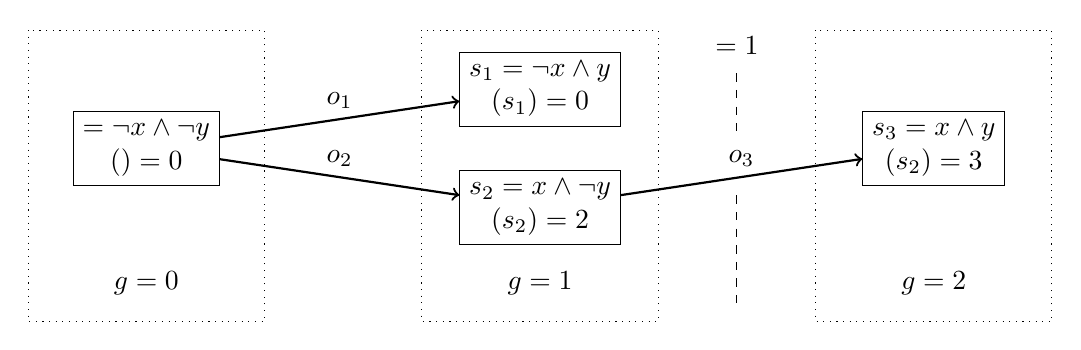
\begin{tikzpicture}[yscale=1]
    \begin{scope}
        \node[align=center,draw] (s0) at (0,0) {$\init = \lnot x \land \lnot y$\\$\utility(\init) = 0$};
        \node[align=center,draw] (s1) at (5,0.75) {$s_1 = \lnot x \land y$\\$\utility(s_1) = 0$};
        \node[align=center,draw] (s2) at (5,-0.75) {$s_2 = x \land \lnot y$\\$\utility(s_2) = 2$};
        \node[align=center,draw] (s3) at (10,0) {$s_3 = x \land y$\\$\utility(s_2) = 3$};

        \draw[dotted] (-1.5,1.5) rectangle (1.5,-2.2) node[pos=.5,align=center] {\\\\\\\\\\\\\\$g = 0$};
        \draw[dotted] (3.5,1.5) rectangle (6.5,-2.2) node[pos=.5,align=center] {\\\\\\\\\\\\\\$g = 1$};
        \draw[dotted] (8.5,1.5) rectangle (11.5,-2.2) node[pos=.5,align=center] {\\\\\\\\\\\\\\$g = 2$};

        \draw[dashed] (7.5,0.95) to (7.5,0.2);
        \draw[dashed] (7.5,-0.6) to (7.5,-2.0);
        \node[align=center] at (7.5,1.3) {$\limit = 1$};

        \draw[->, thick] (s0) to node [above, align=center] {$o_1$} (s1);
        \draw[->, thick] (s0) to node [above, align=center] {$o_2$} (s2);
        \draw[->, thick] (s2) to node [above, align=center] {$o_3$} (s3);
    \end{scope}
\end{tikzpicture}
        }
    \end{center}
    \caption[Visualization of an oversubscription planning task.]{Visualization of the transition system induced by the oversubscription planning tasks $\task$ in \Cref{ex:osp-algorithm} \autocite{speck-katz-aaai2021}.}
    \label{fig:osp-example}
\end{figure}

\section{Symbolic Search}
\textcite{speck-katz-aaai2021} define symbolic \emph{forward} search for osp in a straightforward way and showed that their approach is complete and optimal.
In fact, the presented symbolic search approach finds not only a utility-optimal plan but also a cheapest utility-optimal plan.

The underlying idea is to perform an exhaustive symbolic forward search, just as in classical planning, until the cost bound $\limit$ is exceeded.
The utility function $\utility$ is a numerical function that can be represented with one ADD or several BDDs, as explained in \Cref{ex:dds}.
In each expansion step, the utility of the expanded states is symbolically evaluated and the states with the highest utility so far are maintained.
In addition, representing the utility as ADDs (or BDDs) has the advantage that the highest possible value of the utility function is known directly, since it is simply the terminal node with the highest value.
Finally, we stop when either all reachable states have been expanded within the cost bound or a state with the overall maximum utility has been found, since there can be no better plan.
\Cref{ex:osp-algorithm} illustrates how the symbolic approach of \textcite{speck-katz-aaai2021} works.

\begin{example}[\cite{speck-katz-aaai2021}]\label{ex:osp-algorithm}
    Consider a unit-cost oversubscription planning task $\task = \langle \vars, \operators, \constcostfun, \utility, \init, \goal, \limit \rangle$ with an empty goal $\goal = \{\}$ such that all states are goal states, i.e., $\states = \goalstates$.
    Moreover, $\task$ has two binary variables $\vars = \{x,y\}$, where $\vardomain_x = \vardomain_y = \{0,1\}$, an initial state $\init(x) = \init(y) = 0$, a utility function $\utility = 2x + xy$, and a cost bound $\limit = 1$.
    There exist three operators $O = \{o_1,o_2,o_3\}$, where $o_1 = \langle \lnot x \land \lnot y, y \rangle$, $o_2 = \langle \lnot x \land \lnot y, x \rangle$ and $o_3 = \langle x \land \lnot y, y \rangle$.
    The induced transition system of $\task$ is depicted in Figure \ref{fig:osp-example}.

    Symbolic forward search for osp \autocite{speck-katz-aaai2021} starts with a BDD representing the set of states $open = \{\init\}= \lnot x \land \lnot y$ consisting of a single state, namely the initial state.
    \Cref{fig:add} visualizes the ADD and \Cref{fig:bdd_0,fig:bdd_2,fig:bdd_3} visualize the BDDs representing the utility function $\utility$ with a maximum utility of $3$.
    In the first step, we expand $\{\init\}$, which also forms the set of best states seen so far with utility $\utility(\init) = 0$.
    The expansion leads to two new states $open = \{s_1,s_2\} = (\lnot x \land y) \lor (x \land \lnot y)$, both of which can be achieved with cost $g = 1$.
    Since $s_2$ has utility $\utility(s_2) = 2$, the set of best states changes to $\{ s_2 \}$.
    Finally, the plan $\langle o_2 \rangle$ leading to one of the best states (here $s_2$) is reconstructed as the cost limit of $\limit = 1$ is exceeded.
    Recall that all these computations are performed with decision diagrams.
\end{example}

Finally, \textcite{speck-katz-aaai2021} argue that it is not straightforward to efficiently apply regression to osp, which would enable symbolic backward search and, in particular, symbolic bidirectional search.
Unlike classical planning, where the starting point of symbolic backward search is obvious, namely the goal states represented as a compact goal formula, the starting point of symbolic backward search for osp is not obvious.
%
The reason is that the objective is to find a final state with maximum utility, and it is not clear how this can be represented in backward search.
It might be possible to partition all goal states by their utility values and represent them as separate BDDs.
However, since the goal formula in osp tasks is often unspecified or even empty, this may require a regression of the entire
state space with multiple backward searches.
All in all, it is not clear how to efficiently apply symbolic regression to osp, which is an open research question.

\begin{table}[t]
    \begin{center}
        \resizebox{1\textwidth}{!}{
            \begin{tabular}{lrrrrrrrr}
    \toprule
    Algorithm                    & \multicolumn{2}{c}{\textbf{BDD Search}}   & \multicolumn{1}{c}{\textbf{\astar{uADD}}} & \multicolumn{3}{c}{\astar{mc}}                     & \multicolumn{2}{c}{BnB}                                                                                                                                                                                                              \\
    \cmidrule(lr){2-3} \cmidrule(lr){4-4} \cmidrule(lr){5-7} \cmidrule(lr){8-9}
    Benchmark (\# Tasks)     & \multicolumn{1}{c}{uBDD} & \multicolumn{1}{c}{uADD}                               & \multicolumn{1}{c}{{\heu{blind}{}}} & \multicolumn{1}{c}{\heu{blind}{}} & \multicolumn{1}{c}{\heu{max}{b}} & \multicolumn{1}{c}{\heu{m\&s}{b}} & \multicolumn{1}{c}{\heu{blind}{}} & \multicolumn{1}{c}{\heu{lmcut}{mc}} 
    \\
    \midrule
    ~~25\% Bound (1667) & 1271                                     & \textbf{1274}                                                          & 1165                                                & 1197                                   & 1190                                            & 1074                                             & 1183                                   & 1151                                             \\
    ~~50\% Bound (1667) & 990                                      & \textbf{993}                                                           & 860                                                 & 901                                    & 902                                             & 828                                              & 893                                    & 867                                              \\
    ~~75\% Bound (1667) & \textbf{866}                             & 862                                                                    & 718                                                 & 758                                    & 738                                             & 734                                              & 735                                    & 702                                              \\
    100\% Bound (1667)  & \textbf{802}                             & 793                                                                    & 629                                                 & 668                                    & 655                                             & 676                                              & 643                                    & 618                                              \\
    \midrule
    \textbf{Sum (6668)}      & \textbf{3929}                            & 3922                                                                   & 3372                                                & 3524                                   & 3485                                            & 3312                                             & 3454                                   & 3338                                             \\
    \bottomrule
\end{tabular}

        }
    \end{center}
    \caption[Coverage for oversubscription planning.]{Coverage (number of optimally solved instances) for explicit and symbolic search algorithms on oversubscription planning domains \autocite{speck-katz-aaai2021}.}
    \label{tab:coverage_oversubscription}
\end{table}

\paragraph{Empirical Evaluation.}
\Cref{tab:coverage_oversubscription} shows the coverage on four different osp benchmark sets \autocite{speck-katz-aaai2021}.
Each benchmark set consists of 57 domains and originates from the optimal track of the IPC 1998-2014, where the goal facts are no longer hard goal facts, but have assigned utilities \autocite{katz-et-al-zenodo2019,katz-et-al-icaps2019}.
The sets differ in the cost bounds, which for each planning instance are set at 25\%, 50\%, 75\%, or 100\% of the cost of the optimal or best known solution.
The two symbolic search approaches (BDD search) perform a forward search using BDDs, but differ in how the utility of a set of states is evaluated, either with multiple BDDs (uBDD) or one ADD (uADD).
As a result, symbolic search with a decomposed utility function in multiple BDDs (BDD search + uBDD) works best overall.
The main advantage of representing utility values with BDDs compared to ADDs is that the underlying decision diagram library \name{cudd} \autocite{somenzi-cudd2015} uses techniques such as complement edges to store BDDs more compactly \autocite{brace-et-al-acm1990}.

\begin{figure}
    \begin{center}
        \includegraphics[width=1\textwidth]{pictures/osp_plot.png}
    \end{center}
    \caption[Coverage over time for oversubscription planning.]{Coverage (number of optimally solved instances) over time for explicit and symbolic search algorithms on all oversubscription planning domains (25\%, 50\%, 75\%, or 100\% Bound) \autocite{speck-katz-aaai2021}.}
    \label{fig:coverage_time_oversubscription}
\end{figure}

Overall, the described symbolic search approach \autocite{speck-katz-aaai2021} performs better than explicit search approaches.
Comparing symbolic search with its explicit counterpart, $\astar{uADD}$ search with the blind heuristic \heu{blind}{}, we see a difference in performance due to the concise representation of state sets.
Considering other publicly available planning algorithms for osp, we find that branch-and-bound search BnB \autocite{katz-et-al-icaps2019} and $\astar{mc}$ search with multiple cost functions (mc) \autocite{katz-keyder-icaps2019wshsdip} perform worse than symbolic search in terms of overall coverage.
The performance difference between symbolic search and explicit heuristic search increases as the bound increases and thus the plan length increases.
The natural explanation for this is that heuristics do not pay off, since in osp it seems rather difficult to define a heuristic that is both informative and fast to compute. %, which is why blind heuristics work best.
This observation is underlined by \Cref{fig:coverage_time_oversubscription}, which depicts the number of instances solved over time, where symbolic search dominates all other approaches after a short time.
Finally, as usual, there are domains where explicit heuristic search performs better than symbolic search.


%\section{Summary}
